\chapter{Revisão bibliográfica} \label{chap:revBibli}
	\section{Breve revisão dos conceitos utilizados neste trabalho}


		\begin{figure}
			\centering
			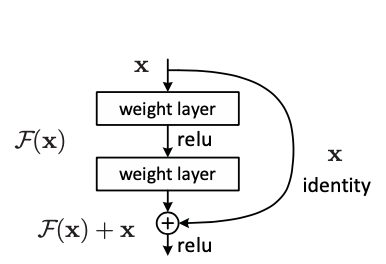
\includegraphics[width=0.7\linewidth]{images/ResidualLearnningBuildBlock}
			\caption[Residual learning: a building block.]{Residual learning: a building block.}
			\label{fig:residuallearnningbuildblock}
		\end{figure}
	
		\par De acordo com \cite{DBLP:journals/corr/HeZRS15} Redes neurais residuais são aquelas que "pulam" algumas camadas, ou seja, a saída de uma camada vai para a próxima mas também vai para uma outra mais à frente. 
		\begin{figure}
			\centering
			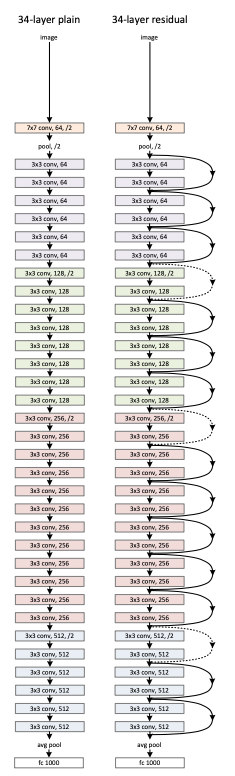
\includegraphics[width=0.3\linewidth]{images/ResidualLearnningNNAndRegularNN}
			\caption[Comparação entre uma rede neural regular e uma rede neural residual]{Comparação entre uma rede neural regular e uma rede neural residual, a direita a rede neural regular percorre sequencialmente todas as suas camadas, a esquerda a rede neural residual "pula" algumas camadas reiteradamente.}
			\label{fig:residuallearnningnnandregularnn}
		\end{figure}
		
		
		
		\subsection{Sinais digitais e sub-amostragem (\textit{downsampling})}
			
		\subsection{Caracterização dos processos de produção da voz humana}
		
	\section{Estado-da-arte em \textit{Imagined Speech}}